\chapter{Implementierung der Betriebssoftware}
Die Betriebssoftware wurde, wie in der Aufgabenstellung festgelegt in C geschrieben.
Hierbei fiel die Wahl auf den Standard C99, der mit einigen sprachlichen
Aktualisierungen gegenüber C89 aufwarten kann. Als Compiler wurde eine Version der
GNU Compiler Collection (GCC) mit einem Backend für AVR-kompatiblen Assembler benutzt.
Außer der C Standard Library und der AVR IO Library besitzt die Software keine externen
Abhängigkeiten im Code.
\section{Die Hauptschleife}
Die Hauptschleife ist in dieser Implementierung eine Endlosschleife, da die Beendigung dieser
Schleife dazu führen würde, dass das System nicht mehr reagiert.
Wie in Abb. \ref{main_loop} zu sehen ist, werden in der Hauptschleife vier wichtige Funktionen
aufgerufen.
\subsection{process\_orders()}
Die process\_\-orders()\--Funktion bearbeitet die Befehle, die bereits in der Queue sind. Dafür holt
sich die Funktion den aktuellen Befehl von der Queue. Falls es solch einen Befehl gibt ruft die
Funktion eine Verteilerfunktion auf. Diese wiederum ruft die zugehörige Befehlsfunktion auf, indem
die untersten vier Bits des ersten Befehlsbytes als Index für eine Call-Table benutzt werden (siehe
Abb. \ref{dispatch_function}).\\
\begin{figure}[htb]
 \centering
 \scalebox{0.5}{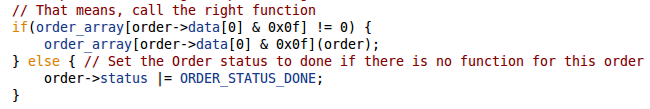
\includegraphics{pictures/dispatch_function.png}}
 \caption{\label{dispatch_function}Die Verteilerfunktion}
\end{figure}
Falls kein Befehl vorliegt oder die Queue angehalten wurde, ruft die process\_\-orders()-Funktion die
Funktion zum aktiven Bremsen auf. Das aktive Bremsen wird in später noch diskutiert.
\subsection{lcd\_update\_screen()}
In dem Fall, dass ein LCD angeschlossen ist, können dort Informationen ausgegeben werden. Ob ein LCD
angeschlossen ist wird über die Stellung eines DIP-Schalters auf der Platine geregelt.\\
Da das synchrone Aktualisieren des LCD sehr viel Zeit benötigt (vgl. <Untersuchung-LCD-Problem>), wird
während dieser Funktion maximal ein Zeichen an das LCD geschickt. Dies wird erreicht indem das Busy-Flag,
welches signalisiert, dass das LCD noch beschäftigt ist, abgefragt wird. Falls es nicht gesetzt ist und
es noch Daten zum aktualisieren gibt, wird das nächste Zeichen an das LCD gesendet.\\
Auf dem LCD werden die Versionsnummer der Betriebssoftware, der Status einiger Systemweiter Variablen und
der aktuelle ausgeführte Befehl angezeigt. Falls nun ein Befehl bearbeitet wird, der länger als einen
Schleifendurchlauf benötigt (das sind z.B. alle Fahr-Befehle), ruft die lcd\_\-update\_\-screen()-Funktion
die lcd\_\-update\_\-info()-Funktion auf, die diese Informationen in einem Puffer konstruiert. Nach und nach
gibt die lcd\_\-update\_\-screen()-Funktion den Inhalt dieses Puffer an das LCD weiter.\\
Befehle die innerhalb eines Hauptschleifendurchlaufs abgearbeitet sind werden nicht ausgegeben und
generieren auch keinen Aufruf von lcd\_\-update\_\-info(). Dies ist nötig, da diese Befehle zu schnell abgearbeitet
werden. Es können vier bis fünf dieser Befehle abgearbeitet werden, bevor das LCD auch nur einmal vollständig
aktualisiert werden kann.
\subsection{parser\_update()}
Der Parser ist dafür zuständig aus den Bytes, die über I2C oder UART gelesen werden, Befehle in Form von
order\_t-Strukturen zu erstellen. Die parser\_\-update()-Funktion fragt beim IO-Modul nach, wieviele Bytes
zum Abholen bereit stehen. Diese werden dann geholt und an die Funktion parser\_\-add\_\-byte() übergeben.\\
Diese parser\_\-add\_\-byte()-Funktion fügt das Byte an die korrekte Stelle im Puffer ein. Wenn ein Befehl
komplett ist, was mit der parser\_\-order\_\-complete()-Funktion überprüft wird, gilt der Befehl als fertig und
alle weiteren Bytes, die hinzugefügt werden, landen in einer neuen order\_t-Struktur.\\
Damit erkannt werden kann, wann ein Befehl zu ende ist benutzt die parser\_\-order\_\-complete()-Funktion
die bytes\_\-needed()-Funktion, in der fest codiert ist, welcher Befehlscode mit welchen Optionen wieviele
Bytes benötigt. Dies ist auch eine der Stellen, die angepasst werden müssen, wenn ein neuer Befehl hinzugefügt
wird, oder bestehende verändert werden.
\subsection{queue\_update()}
\section{Das Aktive Brems System (ABS)}
Das aktive Bremsen steuert die Räder in der Art, dass sie möglichst
auf einem Flecken verweilen. Dazu muss nach dem Ende eines Fahr-Befehls die aktuelle Position der Räder
vermerkt werden, die dann nachher als Referenzpunkt dient.
% Hauptschleife, was wird während der Hauptschleife erledigt
% Datenpfad: Wie laufen die Daten vom Eingang bis zur Verarbeitung
% Debug Define Trick
% Order Type Aufbau und Benutzung, sowie order dispatching
